
\chapter{Controller}
Der Controller bei einem E-Bike spielt eine zentrale Rolle bei der Steuerung des Motors und der Batterie. Seine Hauptfunktionen umfassen:

\begin{enumerate}
  \item \textbf{Leistungsregelung:} Der Controller steuert die Leistungszufuhr zum Motor, was die Geschwindigkeit und Beschleunigung des E-Bikes beeinflusst. Je nach den Einstellungen und Anforderungen des Fahrers kann der Controller die Leistung variieren, um eine sanfte Beschleunigung oder eine schnelle Fahrt zu ermöglichen.

  \item \textbf{Unterstützungsmodi:} Viele E-Bikes bieten verschiedene Unterstützungsmodi, die es dem Fahrer ermöglichen, die gewünschte Leistung und Reichweite auszuwählen. Der Controller steuert diese Modi und passt die Leistung des Motors entsprechend an.

  \item \textbf{Sicherheitsfunktionen:} Der Controller kann Sicherheitsfunktionen wie Überhitzungsschutz und Kurzschlussschutz bieten, um den sicheren Betrieb des E-Bikes zu gewährleisten.
\end{enumerate}

Insgesamt ist der Controller eine wesentliche Komponente eines E-Bikes, die eine präzise Steuerung der Leistung und eine effiziente Nutzung der Batterie ermöglicht.

\section{Controller Parameter}
%Was heißen die Controller Parameter?
%Bild vom Controller
\begin{figure}[h]
  \centering
  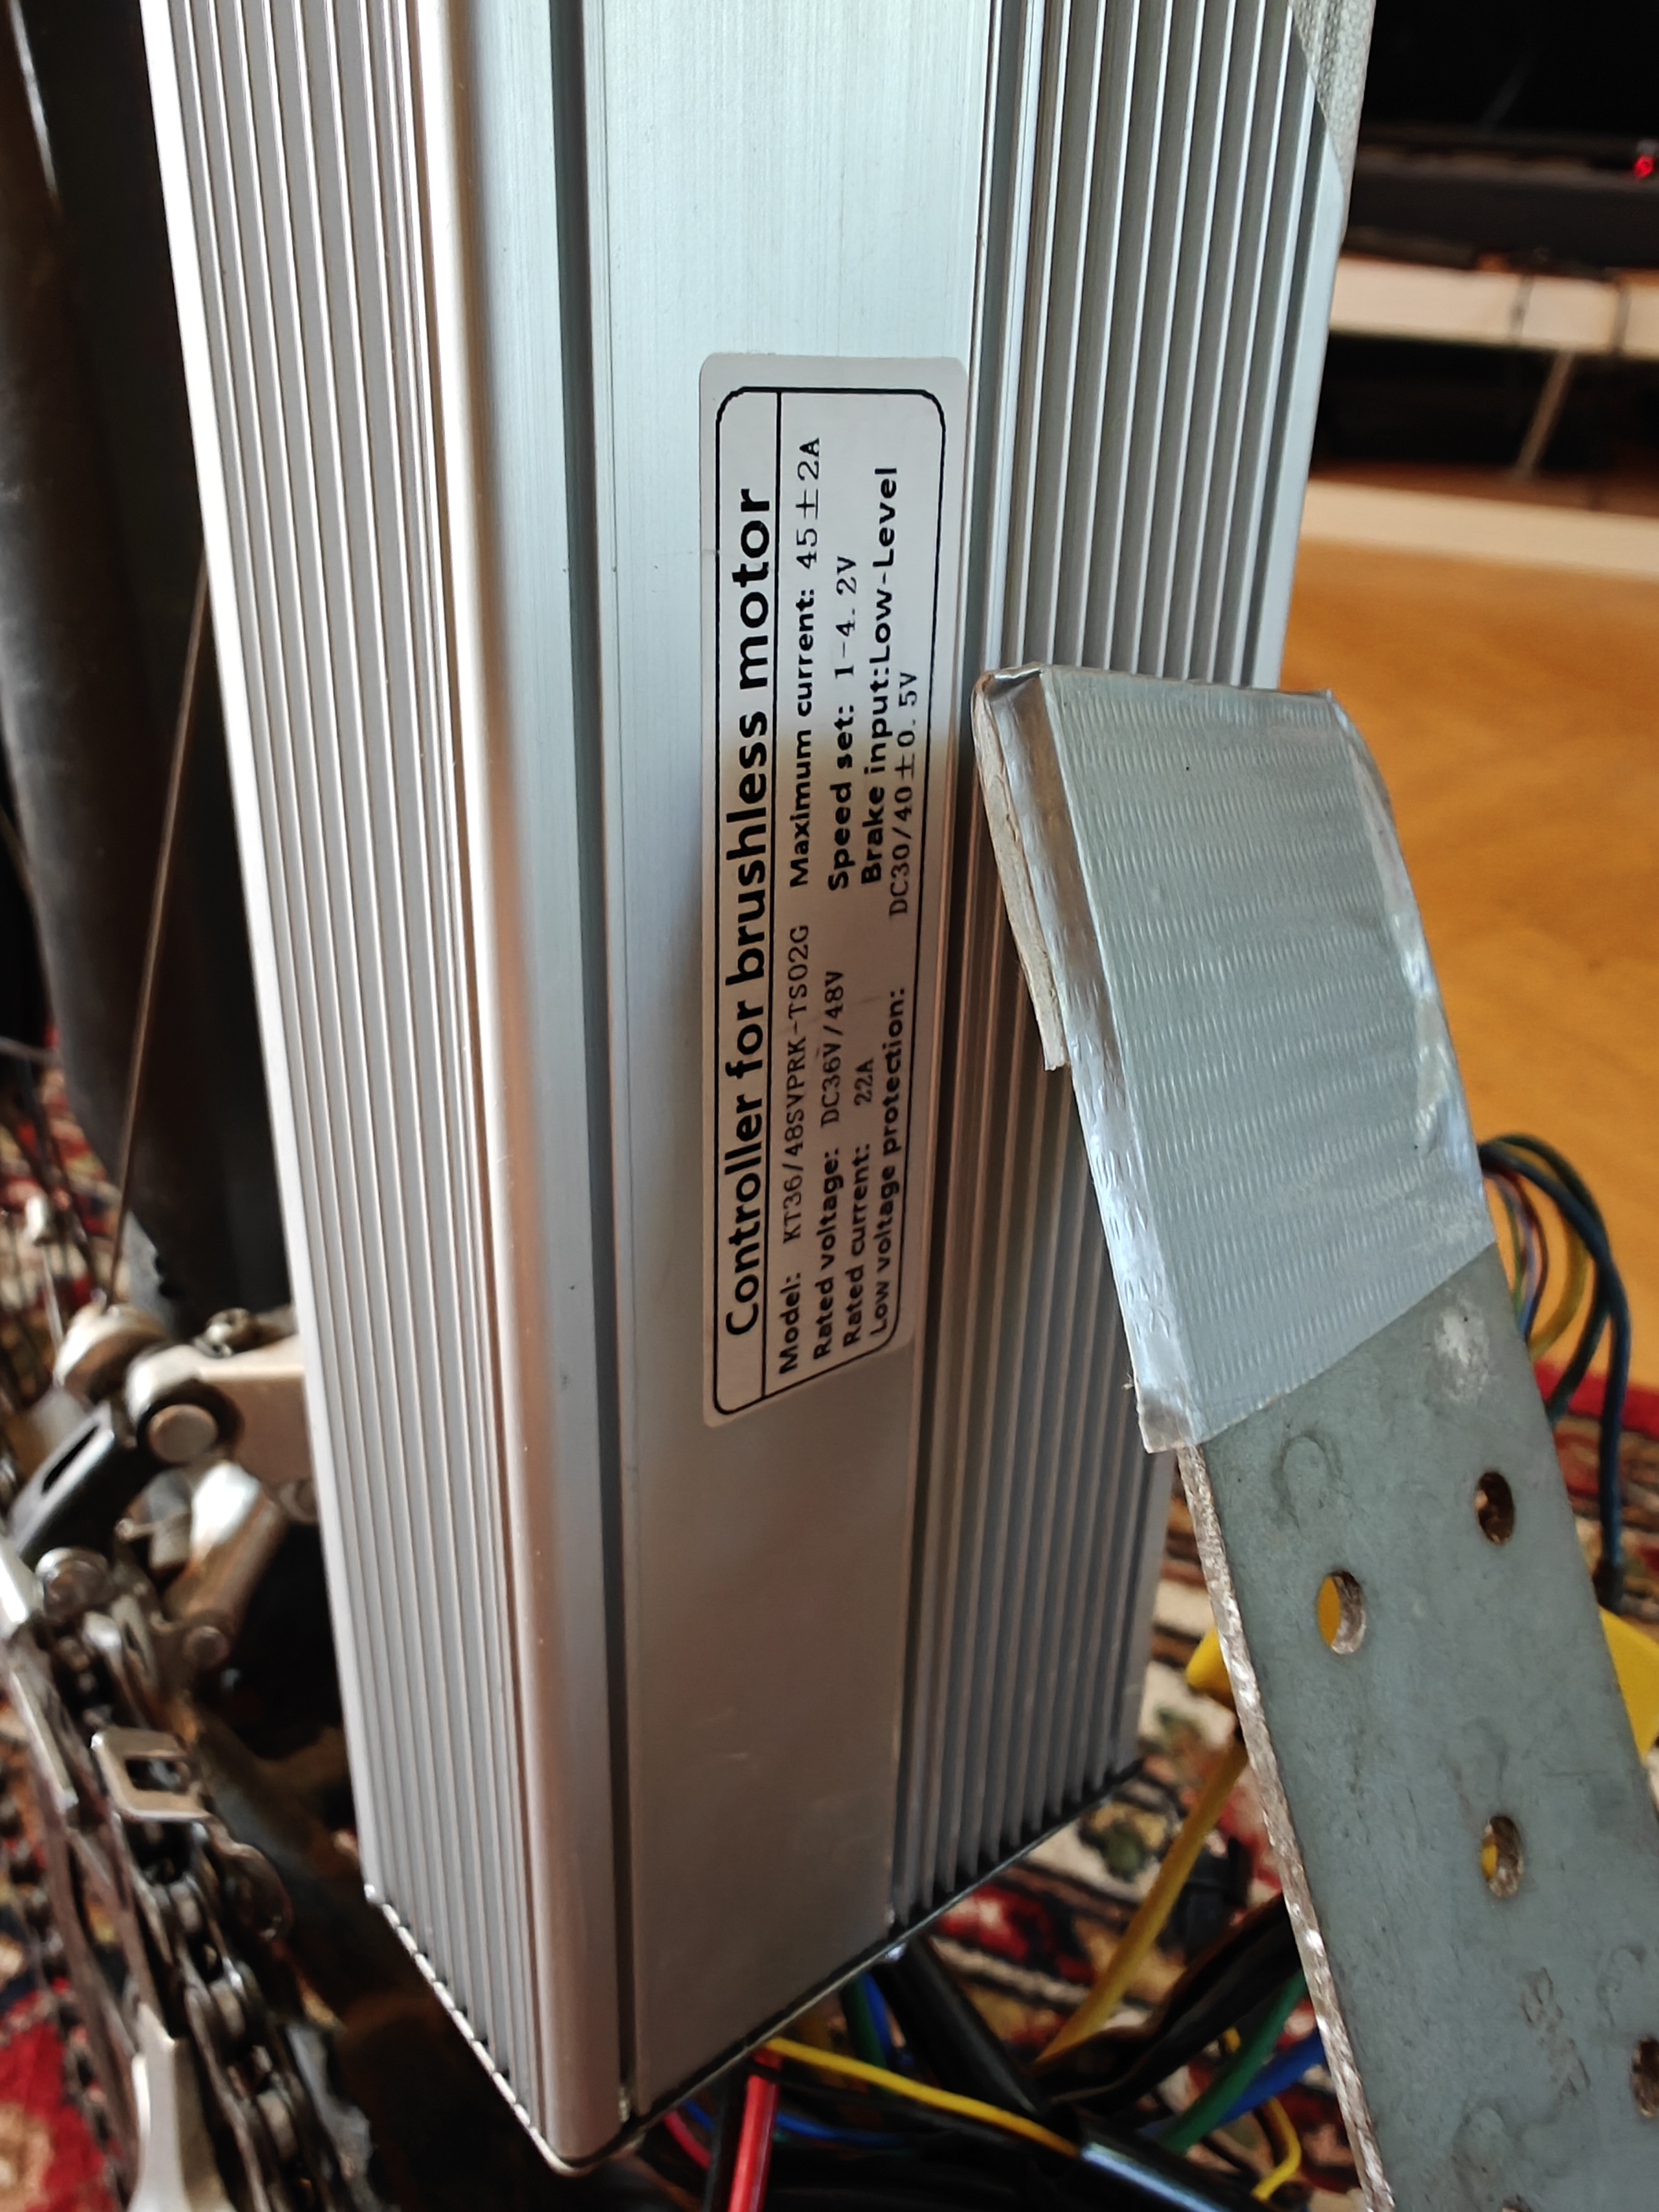
\includegraphics[width=8cm]{images/Controller.jpg}
  \caption{Controller Parameter\cite{lorenz_scherrer_selbst_2023}}%
  \label{fig:17}
\end{figure}

Hier sind einige wichtige Parameter und ihre Bedeutungen \ref{fig:17}:

\begin{enumerate}
  \item \textbf{Rated Voltage (Nennspannung):} Diese Angabe gibt die Spannung an, bei der der Controller ordnungsgemäß funktioniert. In deinem Fall beträgt die Nennspannung DC36V / 48V, was bedeutet, dass der Controller für den Betrieb mit Batterien mit einer Spannung von entweder 36V oder 48V ausgelegt ist.
  
  \item \textbf{Rated Current (Nennstrom):} Dies ist die maximale Stromstärke, die der Controller kontinuierlich liefern kann, ohne überlastet zu werden. Der Nennstrom wird normalerweise in Ampere (A) gemessen und bestimmt die Leistungsfähigkeit des Controllers, den Motor mit Energie zu versorgen.
  
  \item \textbf{Low Voltage Protection (Unterspannungsschutz):} Diese Funktion schützt die Batterie vor übermäßiger Entladung, indem der Controller den Betrieb des Motors abschaltet, wenn die Batteriespannung unter einen bestimmten Schwellenwert fällt. Dadurch wird verhindert, dass die Batterie beschädigt wird und ihre Lebensdauer verlängert.
  
  \item \textbf{Maximum Current (Maximalstrom):} Dies ist die maximale Stromstärke, die der Controller kurzzeitig liefern kann, um beispielsweise bei Beschleunigungsvorgängen einen hohen Drehmoment zu erzeugen. Es ist wichtig, dass dieser Wert die Spezifikationen des Motors und anderer Komponenten nicht überschreitet, um Schäden zu vermeiden.
  
  \item \textbf{Speed Set (Geschwindigkeitseinstellung):} Diese Funktion ermöglicht es dem Benutzer, die maximale Geschwindigkeit des E-Bikes einzustellen. Der Controller regelt dann die Leistung entsprechend, um diese Geschwindigkeit beizubehalten.
  
  \item \textbf{Brake Input (Bremseneingang):} Dieser Eingang ermöglicht es dem Controller, auf Bremsvorgänge zu reagieren, beispielsweise indem er den Motor abschaltet oder die Rückgewinnung von Bremsenergie aktiviert, um die Batterie wieder aufzuladen.
\end{enumerate}

Diese Parameter sind entscheidend für die korrekte Konfiguration und den sicheren Betrieb des E-Bike-Systems und sollten entsprechend den Anforderungen des Fahrzeugs.

\section{Funktionsweise eines Controllers}

%Wie funktioniert ein Controller?

%Gibt es ein Bild von der Reglungstechnik?

%Wie viele Modfet hat dieser Controller? 18



\begin{figure}[h]
  \centering
  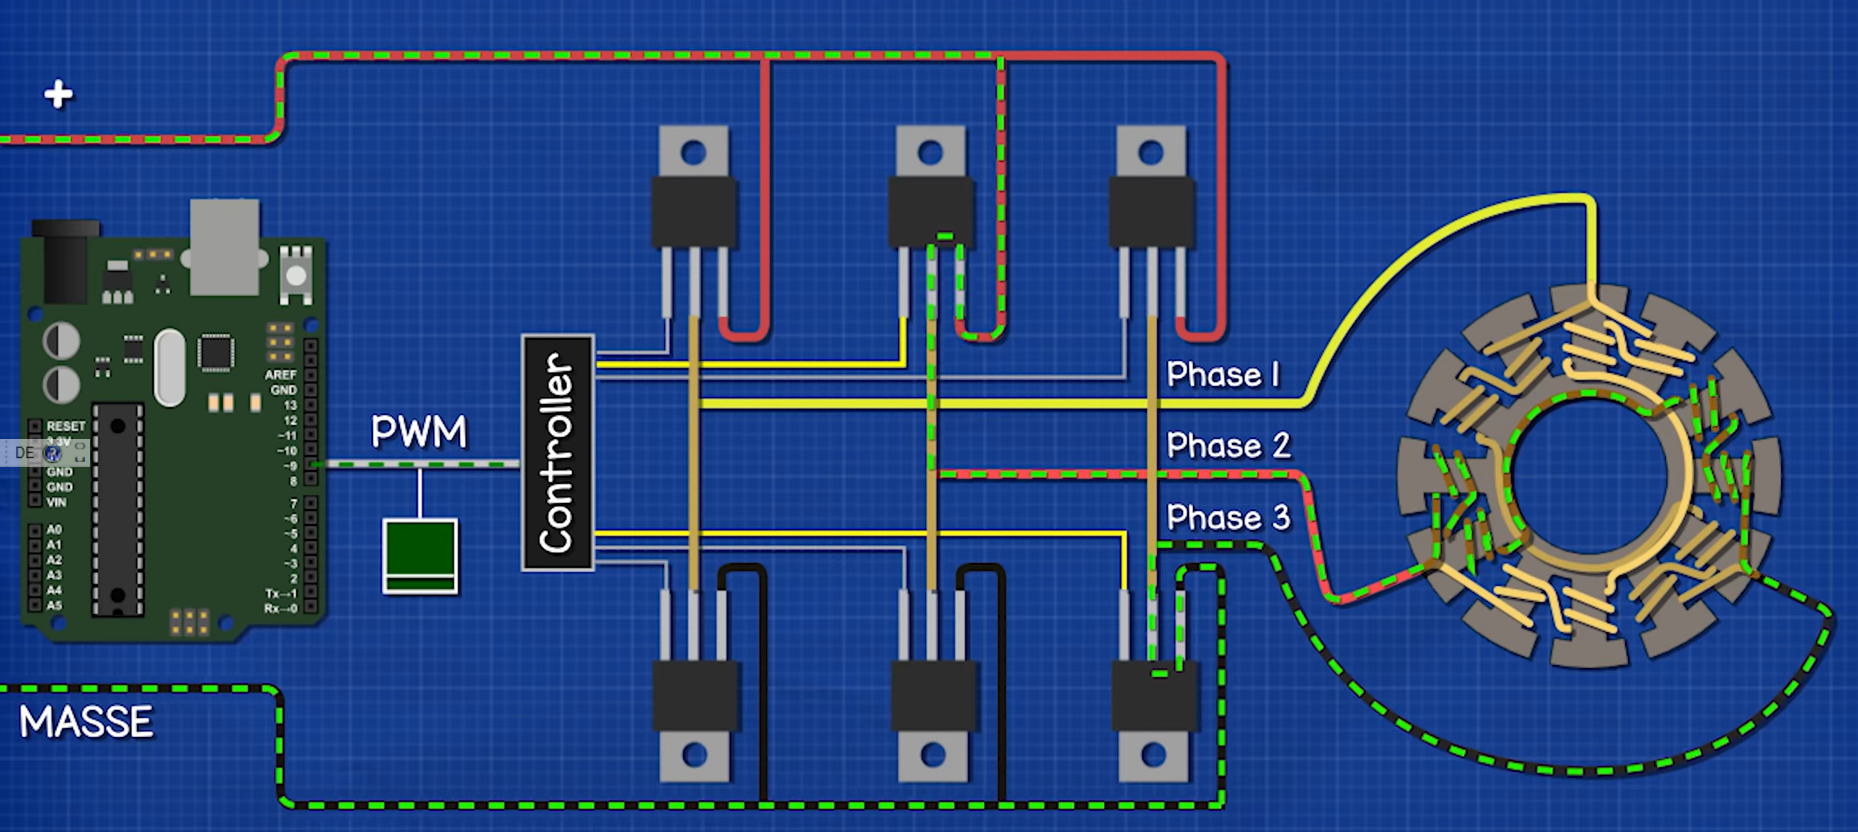
\includegraphics[width=8cm]{images/Funktion der Mosfets.png}
  \caption{Funktionsweise eines Controllers \cite{noauthor_2822_nodate}}%
  \label{fig:18}
\end{figure}

\begin{comment}
\section{Wahl des Controllers}
Vergleich des alten Controller und neuen Controller.
%Welche Funktionen haben die Controller?

%Welche Leistung haben die beiden Controller?

%Wie ist die Größe der beiden Controller?
\end{comment}

\section{Installation des Controllers}

\begin{figure}[h]
  \centering
  \includegraphics[width=8cm]{images/Controller_Anschlüsse.png}
  \caption{Anschlüsse des Controllers\cite{noauthor_2248_nodate}}%
  \label{fig:16}
\end{figure}


Hier ist der Text, der die Anschlüsse des Controllers und ihre Bedeutungen beschreibt, die in diesem Bild zu sehen sind\ref{fig:16}:

\begin{enumerate}
\item \textbf{Phase Hall Sensor Wire (Phasen-Hall-Sensor-Kabel):} Diese Anschlüsse sind für die Verbindung mit den Hall-Sensoren des Motors vorgesehen. Die Hall-Sensoren dienen dazu, die Position des Rotors des Motors zu erfassen und dem Controller mitzuteilen, wann und wie viel Strom an die einzelnen Phasen des Motors geliefert werden soll.

\item \textbf{Battery (Batterie):} Dieser Anschluss ist für die Verbindung mit der Batterie des E-Bikes vorgesehen. Hier wird die Stromversorgung für den Controller und den Motor bereitgestellt.

\item \textbf{Throttle (Gashebel):} Dieser Anschluss ist für die Verbindung mit dem Gashebel des E-Bikes vorgesehen. Der Gashebel ermöglicht es dem Fahrer, die Geschwindigkeit des E-Bikes zu steuern, indem er die Leistung des Motors reguliert.

\item \textbf{PAS Sensor (Pedal-Assist-Sensor):} Dieser Anschluss ist für die Verbindung mit dem Pedal-Assist-Sensor vorgesehen. Der PAS-Sensor erkennt die Pedalbewegungen des Fahrers und passt die Leistung des Motors entsprechend an, um eine unterstützende Fahrt zu gewährleisten.

\item \textbf{Brake Light (Bremslicht):} Dieser Anschluss ist für die Verbindung mit dem Bremslicht des E-Bikes vorgesehen. Wenn der Fahrer bremst, wird das Bremslicht aktiviert, um andere Verkehrsteilnehmer zu warnen.

\item \textbf{Electric Lock (Elektrisches Schloss):} Dieser Anschluss ist für die Verbindung mit dem elektrischen Schloss des E-Bikes vorgesehen. Das elektrische Schloss kann verwendet werden, um das E-Bike vor Diebstahl zu schützen, indem es den Motor oder andere Funktionen sperrt.

\item \textbf{Display (Anzeige):} Dieser Anschluss ist für die Verbindung mit dem Display des E-Bikes vorgesehen. Das Display zeigt dem Fahrer wichtige Informationen wie Geschwindigkeit, Batteriestand und unterstützende Modi an.

\item \textbf{Back-Up (Sicherung):} Dieser Anschluss ist für die Verbindung mit einer Sicherung vorgesehen, um den Controller vor Überlastung oder Kurzschluss zu schützen.

\item \textbf{Cruise Light (Tempomatlicht):} Dieser Anschluss ist für die Verbindung mit einer optionalen Tempomatlichtfunktion vorgesehen, die dem Fahrer anzeigt, wann der Tempomat aktiviert ist.
\end{enumerate}

Diese Anschlüsse ermöglichen es dem Controller, mit verschiedenen Komponenten des E-Bikes zu kommunizieren und sie zu steuern, um eine sichere und effiziente Fahrt zu gewährleisten.

Welche Anschlüsse sind wichtig?
%Es ist möglich den Controller zu programmieren der die Funktiontionen man kann eine Open Sources Software dafür verwenden oder die neue feateurs dafür hinzufügen.
%\url{https://www.pedelecforum.de/wiki/doku.php?id=elektrotechnik:open_source_firmware_fuer_sxxs_ktxx_-controller}
%\url{https://github.com/stancecoke/BMSBattery_S_controllers_firmware/wiki}